\section{Mobilna turystyka}
\nextoc

\subsection{Informacje ogólne}
\begin{frame}
    \frametitle{Informacje ogólne}

\begin{columns}
\column{0.45\textwidth}
Nanoszenie na obraz otaczającego nas miejsca: 
\begin{itemize}
\item Informacje o zabytkach z Wikipedii
\item Szczegóły restauracji, klubów i innych miejsc publicznych
\item Społeczne akcje naszych znajomych z Facebooka, Twittera, itp.
\end{itemize}
\column{0.45\textwidth}
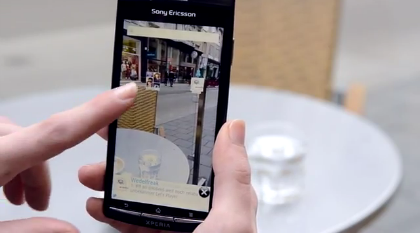
\includegraphics[width=\textwidth]{tourism_1}
\end{columns}
\end{frame}

\subsection{Aplikacje}
\subsubsection{Wikitude}
\begin{frame}[allowframebreaks]
\frametitle{Wikitude}

\begin{columns}
\column{0.45\textwidth}
Informacje ogólne: 
\begin{itemize}
\item Dostepna na Androida i iOS.
\item Darmowa.
\item Miejsca dodawane przez społeczność.
\item Polskie lokacje.
\end{itemize}
\column{0.45\textwidth}
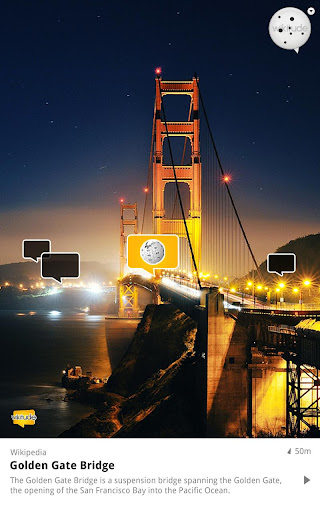
\includegraphics[width=0.8\textwidth]{wikitude}
\end{columns}

\framebreak

Cechy aplikacji:
\begin{itemize}
\item Dostępne ponad 100 milionów miejsc.
\item Wyświetlanie: wpisów Twittera, artykułów z Wikipedii, bankomatów,
    restauracji, opini użytkowników i wydarzeń.
\item Dostępne kupony i rabaty.
\end{itemize}

\end{frame}
\subsubsection{Nearest Tube}
\begin{frame}
\frametitle{Nearest Tube}
Aplikacja pozwalająca znaleźć najbliższe stacje metra w Londynie.
\vspace*{1cm}
\begin{columns}
\column{0.45\textwidth}

Cechy: 
\begin{itemize}
\item Dostepna na tylko iOS.
\item Oznaczanie odległości do stacji metra, a także kierunki 'Jak dojść?'.
\end{itemize}
\column{0.45\textwidth}
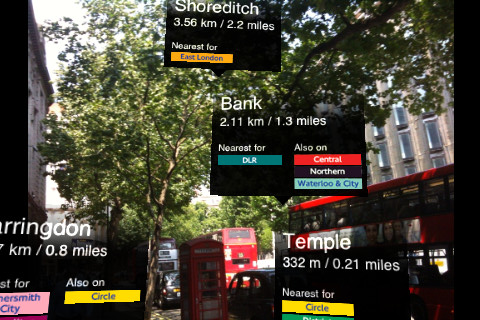
\includegraphics[width=0.8\textwidth]{nearest_tube}
\end{columns}
\end{frame}

\subsection{Podsumowanie}
\begin{frame}
\frametitle{Podsumowanie}
Zalety:
\begin{itemize}
    \item Ułatwienie poruszania się po obcym mieście.
    \item Aplikacje darmowe i dostępne.
    \item Tworzone przez użytkowników.
\end{itemize}
Wady:
\begin{itemize}
    \item Wymaga włączonego GPS i kompasu oraz stałego dostępu do sieci
        Internet.
\end{itemize}
\end{frame}
